
\begin{frame}[fragile,t]
\frametitle{Dynamic Memory Is Hard}
\framesubtitle{``If you write C-style code, you expect to have C-style problems'' -- Stroustrup}

{\scriptsize \begin{verbatim}
void foo() {
  double* d = new double[70];
  ...
  if (condition1)
    return;              // Leak!
  ...
  if (error)
    throw exeption_type;  // Leak!

  foo()           // if an exception happens
                  // in here -- Leak!

  delete d;      // cleanup (?)
}
\end{verbatim}}
\end{frame}




%%%%%%%%%%%%%%%%%%%%%%%%%%%%%%%%%%%%%%%%%%%%%%%%%%%%%%%%%%%%%%%%%%%%%%
\begin{frame}[fragile,t]
\frametitle{SESE}

Single-Entry-Single-Exit is an attempt to mitigate this problem:
\vskip 6pt

\begin{columns}[t]
\column{.5\textwidth}
Heavily nested if-blocks:
{\scriptsize\begin{verbatim}
void foo() {
  if (precondition1) {
    double* d = new double[70];
    if (d) {
      ...
      if (precondition2) {
        Widget* w = new Widget;
        if (w) {
           // finally do some work
           FiddleWidget(w, d);
           ...
           }
        delete w;
        }
     }
   delete d[];
   }
  return;
}
\end{verbatim}}
\pause{}
\column{.5\textwidth}
And doesn't help anyway
{\scriptsize\begin{verbatim}


// Can throw in C++11



// ... might throw



// might throw






\end{verbatim}}
\end{columns}
\pause{}
\vskip 6pt
In the presence of exceptions, \Emph{every function call} can exit the function
\end{frame}


%%%%%%%%%%%%%%%%%%%%%%%%%%%%%%%%%%%%%%%%%%%%%%%%%%%%%%%%%%%%%%%%%%%%%%

\begin{frame}[fragile,t]
\frametitle{Exceptions Break Things}
\framesubtitle{If you don't know what you're doing}
In the presence of exceptions, writing code the old way is nearly impossible:
{\scriptsize\
\begin{verbatim}
void foo() {
  try {  double* d = new double[70]; }
  catch (...) {...}
  ...
  try { foo(); }
  catch (...) { delete d; ...}

  try { bar(); } 
  catch (...) { delete d; ...}

  delete d;      // cleanup
}
\end{verbatim}
}
Every statement must be wrapped in a try/catch block... this is part
of the reason exceptions have a bad rap in C++.
\vskip 6pt
(If you're handling exceptions by writing try and catch everwhere,
you're doing it wrong -- but that's another talk)
\end{frame}

%%%%%%%%%%%%%%%%%%%%%%%%%%%%%%%%%%%%%%%%%%%%%%%%%%%%%%%%%%%%%%%%%%%%%%

\begin{frame}[fragile,t]
\frametitle{}
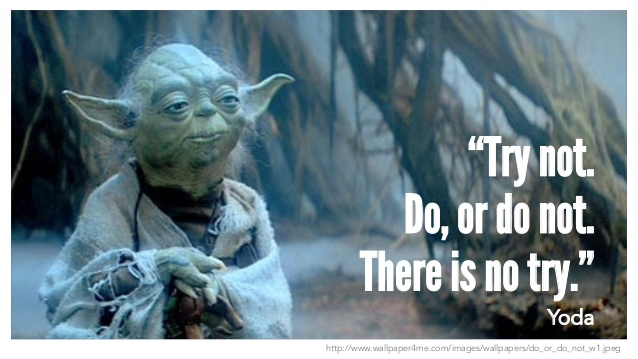
\includegraphics[scale=0.5]{yoda.jpg}
\begin{center}
Many (most?) C++ code bases \emph{do not use exceptions}, including
Google's, and including ours.
\vskip 6pt
\Emph{Writing code \emph{as if} exceptions exist makes code better.}
\end{center}
\end{frame}

\begin{frame}[fragile,t]
\frametitle{A Rant}
\framesubtitle{Before we go on...}
A side note: there is something very wrong here:
\pause{}
{\scriptsize \begin{verbatim}
void foo() {

  Widget* w = new Widget;
  ...
  if (condition1)
    return;       // Leak!
  ...
  if (error)
    throw ex;     // Leak!

  foo()           // an exception happens
                  // in here -- Leak!

  delete w;      // cleanup 
}
\end{verbatim}}
\pause
There's no need to dynamically allocate \texttt{w} in the first place.
\vskip 6pt
\Emph{This isn't Java, so stop it.}

\end{frame}

\begin{frame}[fragile,t]
\frametitle{A Rant}
\framesubtitle{Before we go on...}
Don't hit the heap if you don't have to!

{\scriptsize \begin{verbatim}
void foo() {

  Widget w;      // On the stack!
  ...
  if (condition1)
    return;       // nothing to leak
  ...
  if (error)
    throw ex;     // no problems

  foo()           // an exception happens in here... ok
}
\end{verbatim}}
\pause{}
\begin{itemize}
\item Save runtime
\item Reduce pressure on the heap
\item Reduce memory fragmentation
\pause{}
\item \Emph{Repent, ye Java programmers}
\end{itemize}

\end{frame}

%%%%%%%%%%%%%%%%%%%%%%%%%%%%%%%%%%%%%%%%%%%%%%%%%%%%%%%%%%%%%%%%%%%%%%%%%%%%%%%%

\begin{frame}[fragile,t]
\frametitle{Why dynamic memory at all?}
\center{When must we hit the heap?}
\vskip 6pt
\pause{}

\begin{enumerate}
\item We don't know how many we need until runtime
{\scriptsize \begin{verbatim}
int n;
cin >> n;
Widget* widgets = new Widget[n];
\end{verbatim}
}
\pause{}
\item We don't know what type we need until runtime (polymorphism)
{\scriptsize \begin{verbatim}
class DooDad : public Widget {};
class DooHickey : public DooDad {};
class Gadget : public Widget{}
class Thingy : public Gadget{};

Widget* widget = WidgetFactory(...);
\end{verbatim}
}
\pause{}
\item We don't know how long it's going to live (special case of \#1)
\item Rare corner cases (arcane, nefarious, and sometimes dastardly).
\end{enumerate}

\vskip 12pt
\pause{}

\center{ \Emph{Dynamically allocate only when absolutely necessary} }
\end{frame}
